\documentclass[11pt]{article}

\usepackage[margin=1in]{geometry}
\usepackage{graphicx}
\usepackage{booktabs}
\usepackage{amsmath}
\usepackage{hyperref}
\usepackage{xurl}
\usepackage{caption}
\usepackage{float}
\usepackage{enumitem}
\usepackage{microtype}

\hypersetup{
  colorlinks=true,
  linkcolor=blue,
  urlcolor=blue,
  citecolor=blue
}

\title{Retail Demand Forecasting with Temporal Deep Learning on Walmart M5 Sales Data}
\author{INDENG 242B Final Project}
\date{Spring 2026}

\begin{document}
\maketitle

\begin{abstract}
Retailers rely on short-term demand forecasts to decide how much inventory to replenish, where to allocate labor, and when to investigate possible stockout risk. This project studies daily retail demand forecasting using the public M5 Forecasting dataset, which contains Walmart item-level sales and calendar information. We aggregate item-level sales into 70 operational time series, one for each store-department pair, and train models to predict next-day unit demand from rolling sales histories and calendar covariates. We compare two simple retail forecasting baselines, a lag-based neural network, a temporal Transformer trained from scratch, and reversible instance normalization (RevIN) variants of both neural models. After bounded hyperparameter tuning, the Lag MLP + RevIN model achieves the lowest mean absolute error on the final 56-day validation period. RevIN improves both neural architectures, suggesting that local window normalization is useful for nonstationary retail demand.
\end{abstract}

\section{Project Motivation and Use Case}

Retail demand forecasting is a practical operations problem. A retailer must decide how much product to stock before actual customer demand is observed. If forecasts are too low, shelves may be empty and customers may leave without buying. If forecasts are too high, the retailer may hold excess inventory, waste labor and storage space, or discard perishable goods. These decisions affect revenue, customer experience, logistics cost, and sustainability.

The use case for this project is a department-level planning tool for a large retailer. Given recent sales history and calendar information, the model estimates tomorrow's demand for each store-department pair. Such forecasts could support replenishment planning, staffing, inventory monitoring, and exception reporting. The project is intentionally scoped to an operational level that is meaningful but computationally feasible for a course project. Instead of forecasting every individual product, we aggregate sales by store and department. This reduces noise, allows one model to learn across related time series, and creates forecasts that can be used by a department manager or supply planning team.

\section{Data Source and Learning Problem}

The data source is the M5 Forecasting - Accuracy dataset, originally released through Kaggle and mirrored publicly on Zenodo. The dataset contains daily unit sales for Walmart products across stores from 2011-01-29 through 2016-04-24, along with calendar variables such as weekday, month, events, and SNAP indicators. We use \texttt{sales\_train\_validation.csv} and \texttt{calendar.csv}. The public mirror used for the project is \url{https://zenodo.org/records/12636070}, and the original competition page is \url{https://www.kaggle.com/c/m5-forecasting-accuracy}.

The raw data contains thousands of item-store time series. To create a tractable but realistic forecasting task, we aggregate item-level daily sales into 70 store-department series: 10 stores times 7 departments. For each series, the target variable is daily unit demand. Each supervised training example is created with a rolling window. The input is recent historical demand and associated calendar features, and the label is the next day's demand. Hyperparameter tuning considers 56-, 84-, and 112-day lookback windows; the final MLP family uses 84 days, while the final Transformer family uses 56 days.

Formally, for store-department series $s$ and day $t$, the model learns a function
\begin{equation}
    y_{s,t} = f_{\theta}\left(y_{s,t-L:t-1}, c_{s,t-L:t-1}, c_{s,t}, s\right),
\end{equation}
where $y_{s,t}$ is daily unit demand, $c$ contains calendar covariates, $s$ identifies the store-department series, and $L$ is the tuned lookback length. The final 56 days are held out for validation. The original neural models normalize each series using its training-period mean and standard deviation so that departments with very different demand levels can be learned by a single global model. The RevIN variants additionally normalize each rolling input window using only that window's mean and standard deviation.

The main calendar features are day-of-week sine and cosine terms, month sine and cosine terms, an event indicator, and the state-specific SNAP indicator. The use of cyclic sine and cosine variables avoids treating Sunday and Monday or December and January as artificially far apart.

\section{Methodology}

We train and evaluate six models: two operational baselines, two neural network models, and RevIN variants of both neural networks.

The first baseline is seasonal naive. It predicts that tomorrow's demand will equal demand from the same weekday one week earlier. This is a useful retail baseline because store traffic and shopping behavior often have strong weekly seasonality.

The second baseline is a 28-day moving average. It predicts tomorrow's demand as the average demand over the previous 28 days. This baseline captures the recent demand level while smoothing short-term noise.

The first neural model is a lag MLP, or multi-layer perceptron. The MLP receives normalized lagged sales values as a fixed vector, current calendar features, and a learned series embedding. The series embedding allows the model to learn persistent differences between store-department pairs. The input is passed through fully connected layers with ReLU activations and dropout, and the output is a one-step-ahead normalized demand prediction. This model treats the lag window as a fixed feature vector; it does not explicitly use self-attention, but each lag position has a consistent meaning.

The advanced model is a temporal Transformer encoder trained from scratch. Instead of flattening the history, the Transformer reads it as an ordered sequence. For each day in the lookback window, the model receives normalized demand and calendar features. Positional embeddings encode the order of days in the sequence, and a learned series embedding is added so the model can share information across series while preserving store-department identity. The self-attention layers allow the model to learn which previous days are most useful for predicting the next day. For example, the model can attend to the same weekday one week earlier, recent demand changes, event days, or longer-term patterns within the lookback history.

We add reversible instance normalization (RevIN) as an additional time-series normalization experiment. For each training example, RevIN computes the mean and standard deviation of the input window, normalizes the input window using those statistics, trains the model to predict the next day in this local normalized space, and then reverses the transformation:
\begin{equation}
    \hat{y}_{s,t} = \hat{z}_{s,t}\sigma_{s,t-56:t-1} + \mu_{s,t-56:t-1}.
\end{equation}
Only the input window statistics are used, so the target day is never leaked into the features. We also provide the local mean and standard deviation as auxiliary features so the models can still use information about the local demand level.

Both neural models are trained to minimize mean absolute error on normalized demand. The optimization problem is
\begin{equation}
    \min_{\theta} \frac{1}{N}\sum_{i=1}^{N} \left|f_{\theta}(X_i)-Y_i\right| + \lambda\|\theta\|_2^2,
\end{equation}
where $X_i$ is the input window and calendar information, $Y_i$ is the normalized next-day demand, and the regularization term is implemented through AdamW weight decay. Dropout is also used as regularization. After training, predictions are transformed back into original unit-sales scale for evaluation.

\section{Experimental Setup}

The data is split chronologically. All models train on the earlier portion of the time series and validate on the final 56 days. This avoids leakage from future demand into past forecasts. After adding RevIN, both neural model families are tuned with a bounded sweep over lookback length, learning rate, model width/depth, dropout, and embedding size. The final MLP configuration uses an 84-day lookback, hidden layers 384 and 192, dropout 0.15, embedding size 24, and learning rate 0.0007. The final Transformer configuration uses a 56-day lookback, model dimension 96, four attention heads, two encoder layers, dropout 0.15, and learning rate 0.0007. Final training uses batch size 512, AdamW optimizer, 10 epochs, and validation model selection based on mean absolute error.

We evaluate models using mean absolute error (MAE), root mean squared error (RMSE), symmetric mean absolute percentage error (sMAPE), and weighted absolute percentage error (WAPE). MAE is the primary metric because it has a direct operational interpretation: average absolute unit-sales error per store-department day. RMSE penalizes large errors more heavily, while sMAPE and WAPE provide percentage-style measures that are easier to compare across scales.

\begin{table}[H]
\centering
\caption{Validation performance on the final 56 days.}
\label{tab:metrics}
\begin{tabular}{lrrrr}
\toprule
Model & MAE & RMSE & sMAPE (\%) & WAPE (\%) \\
\midrule
Lag MLP + RevIN & 52.914 & 90.672 & 12.66 & 8.79 \\
Lag MLP & 53.982 & 93.920 & 12.77 & 8.97 \\
Temporal Transformer + RevIN & 56.616 & 99.007 & 12.87 & 9.41 \\
Temporal Transformer & 59.180 & 107.437 & 13.18 & 9.83 \\
Seasonal naive & 86.069 & 158.331 & 18.53 & 14.30 \\
Moving average 28 & 104.758 & 180.311 & 18.94 & 17.40 \\
\bottomrule
\end{tabular}
\end{table}

\begin{figure}[H]
\centering
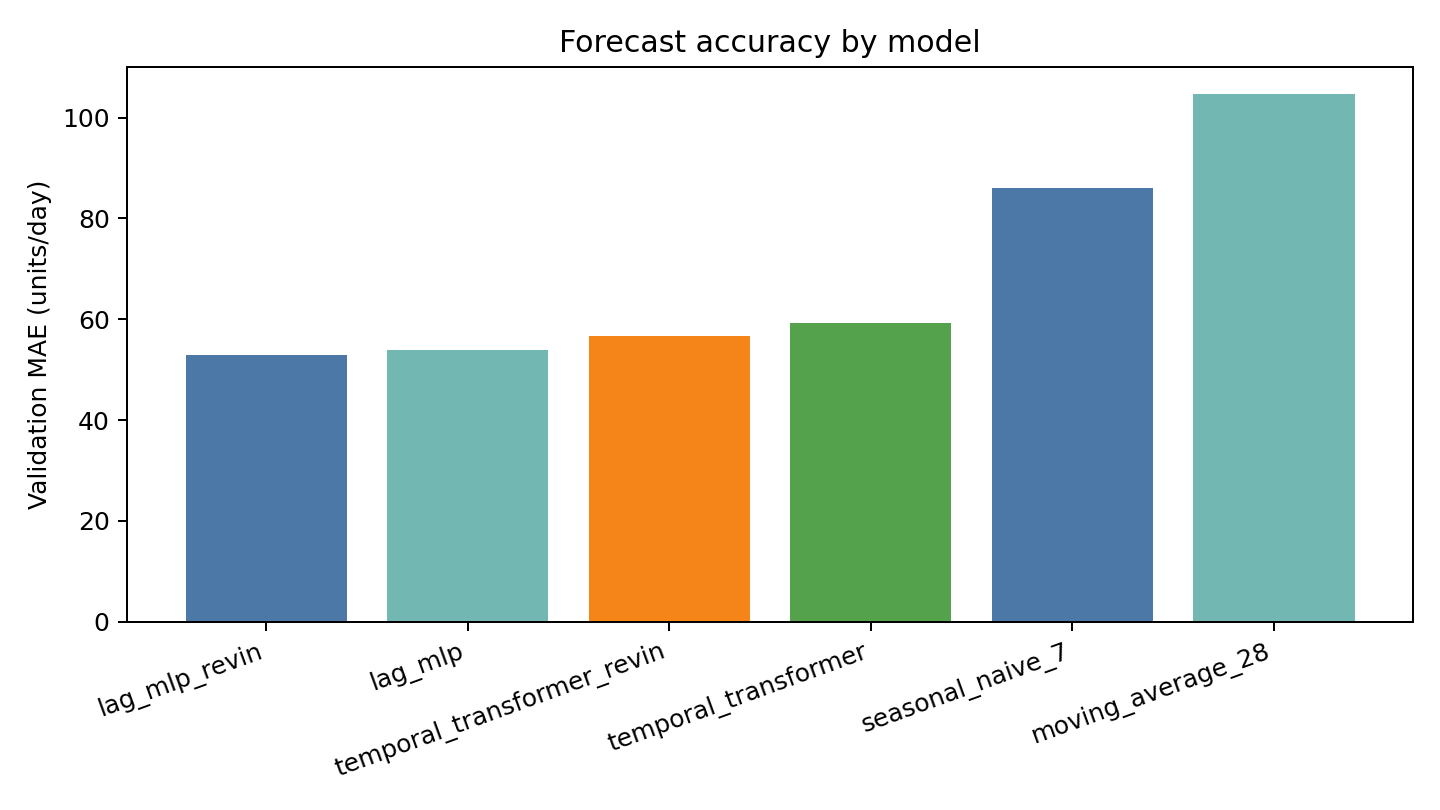
\includegraphics[width=0.78\linewidth]{figures/model_mae_comparison.png}
\caption{Validation MAE comparison across baselines and neural models.}
\label{fig:model-comparison}
\end{figure}

\section{Results and Discussion}

All neural models outperform the simple operational baselines by a substantial margin. The Lag MLP + RevIN model achieves the best validation MAE of 52.91 units per store-department day and WAPE of 8.79 percent. Compared with seasonal naive, which has MAE 86.07, Lag MLP + RevIN reduces MAE by about 39 percent. RevIN also improves the Transformer, reducing MAE from 59.18 to 56.62. The moving-average baseline performs worst, suggesting that simple smoothing loses important weekly and recent-demand structure.

The most important result is that RevIN improves both neural architectures. This supports the hypothesis that local distribution shifts matter in retail demand forecasting. The advanced temporal Transformer improves substantially over non-neural baselines, and the RevIN Transformer closes part of the gap to the MLP. However, it still does not outperform Lag MLP + RevIN in this configuration. This suggests that for aggregated department-level forecasts, recent lag values and local demand level contain enough signal for a compact feed-forward neural network to perform very well.

\begin{figure}[H]
\centering
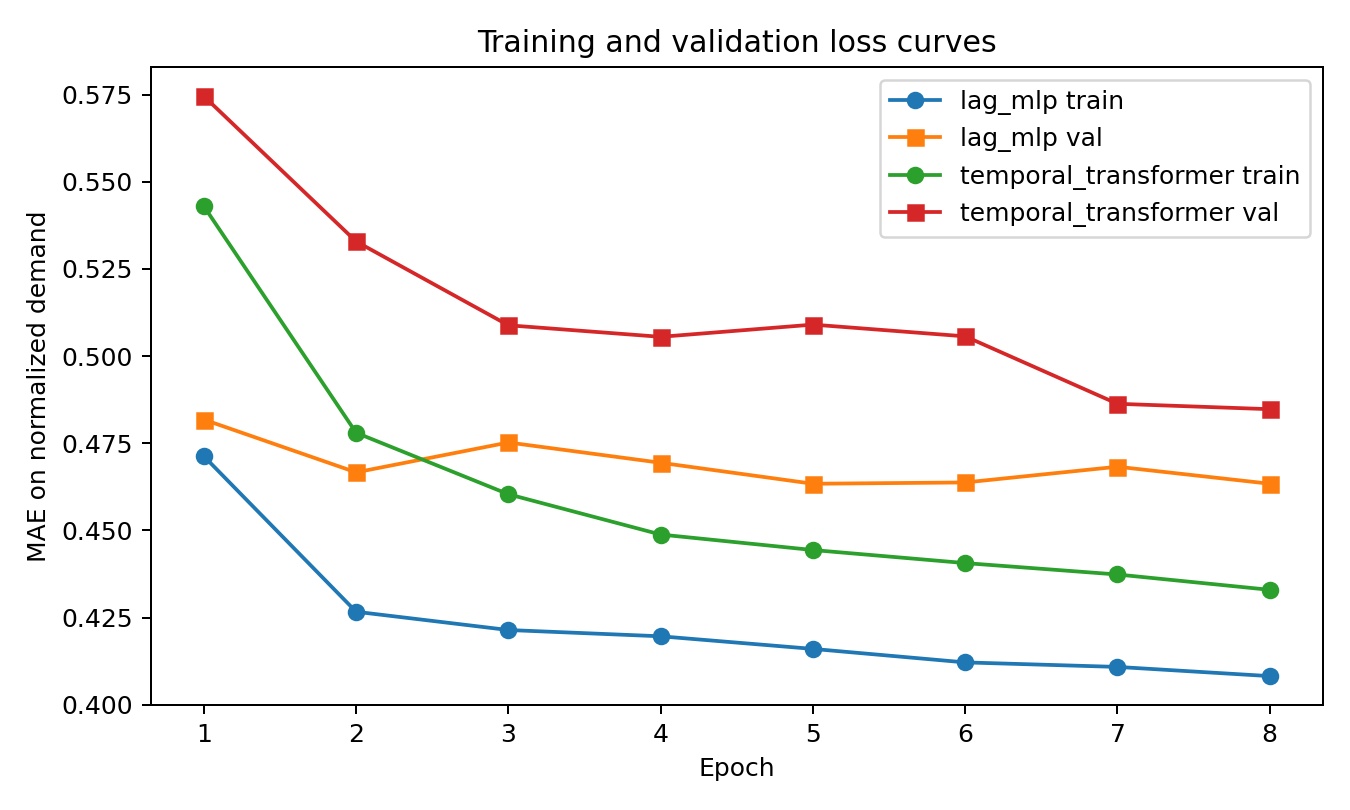
\includegraphics[width=0.78\linewidth]{figures/training_curves.png}
\caption{Training and validation loss curves for the neural models.}
\label{fig:training-curves}
\end{figure}

The training curves show that the lag MLP converges quickly and that RevIN provides a consistent validation improvement. The Transformer continues improving over epochs, and the RevIN Transformer is better than the standard Transformer. This pattern does not indicate a failed Transformer; rather, it shows that higher-capacity attention models are not automatically better for every forecasting problem. Model choice should be evaluated empirically against strong baselines and normalization choices.

\begin{figure}[H]
\centering
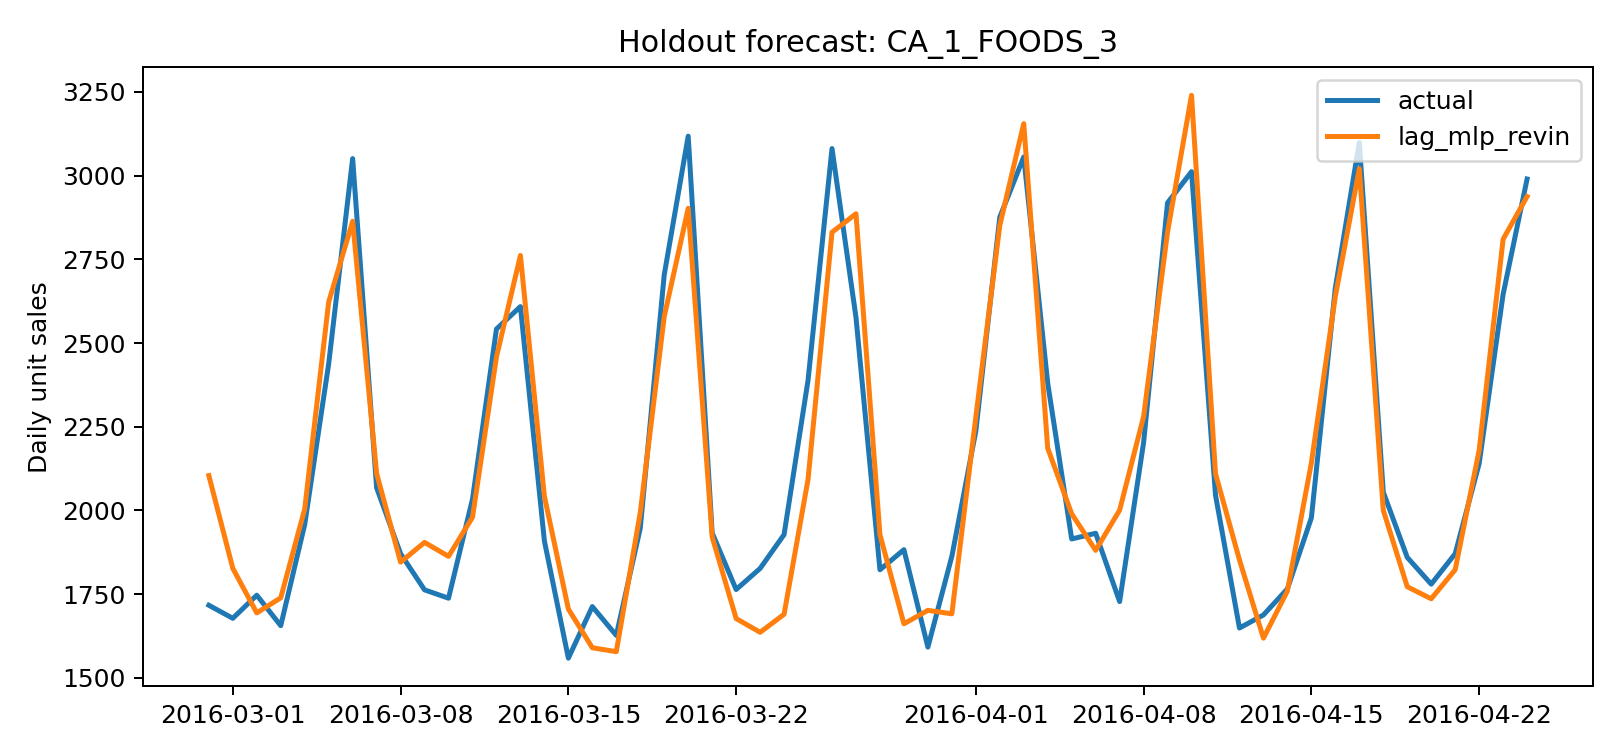
\includegraphics[width=0.78\linewidth]{figures/forecast_CA_1_FOODS_3.png}
\caption{Example holdout forecast for a high-volume food department series.}
\label{fig:forecast-example}
\end{figure}

Example forecast plots for high-volume food departments show that the neural models capture broad demand levels and many short-term fluctuations. Large spikes remain difficult. These spikes may correspond to promotions, stockout recovery, holidays, local events, or other shocks not fully represented by the available calendar variables. Including sell-price features from \texttt{sell\_prices.csv} and explicit promotion information would likely improve spike prediction.

\begin{figure}[H]
\centering
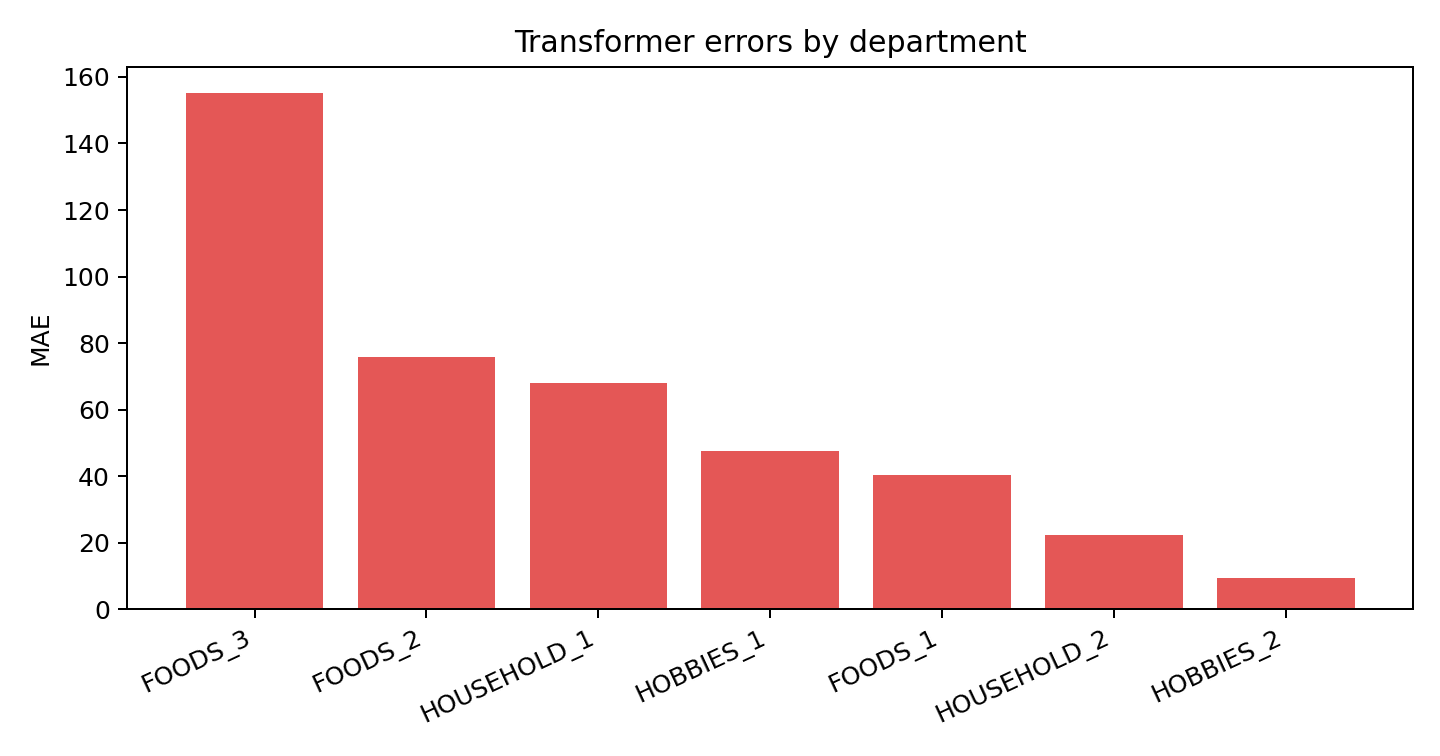
\includegraphics[width=0.70\linewidth]{figures/transformer_mae_by_department.png}
\caption{Transformer validation MAE by department.}
\label{fig:dept-errors}
\end{figure}

\section{Safety, Security, and Ethics}

A retail forecasting model should not directly automate replenishment decisions without guardrails. Forecast errors can create stockouts for essential goods or excess inventory for perishable goods. Stockouts can disproportionately affect customers with fewer shopping alternatives, while overstock can create waste and unnecessary transportation emissions. Because this project forecasts at the department level, it should be used as a planning signal rather than a final ordering decision.

Historical sales may also understate true demand when products were out of stock. If the store had no inventory, observed sales are zero even if customers wanted to buy the product. A model trained only on observed sales may learn to forecast artificially low demand in settings where past stockouts occurred. This is a common safety issue in demand forecasting: sales are not always equal to demand.

The model may also encode regional and socioeconomic demand patterns. Calendar variables such as SNAP indicators can improve forecast accuracy, but they also represent public-benefit timing and should be handled carefully. A deployed model should not be used to reduce service quality in certain locations or to manipulate availability around benefit cycles. It should include human review, service-level constraints, uncertainty estimates, and monitoring for drift after holidays, economic shocks, assortment changes, or supply disruptions.

Security concerns are also relevant. Demand forecasts can reveal commercially sensitive information, including product velocity, regional demand, promotion effects, and inventory constraints. If forecasts are exposed through an internal dashboard, access control and aggregation thresholds should be used to prevent misuse.

\section{Conclusion}

This project builds a complete data-to-model pipeline for practical retail demand forecasting. We use the public M5 Walmart sales dataset, aggregate item-level sales into 70 store-department time series, create rolling-window supervised learning examples, and train our own neural forecasting models. The best model is Lag MLP + RevIN, which outperforms seasonal naive, moving-average, standard MLP, and standard Transformer models on the final 56-day validation period. The temporal Transformer is a meaningful advanced methodology and also improves substantially over simple baselines; adding RevIN further improves it.

The main lesson is that neural forecasting can add value over simple rules, but model complexity and normalization choices must be justified by validation performance. For this aggregated demand task, a compact lag-based neural model with RevIN is strongest. Future work should add price features, train at item-store granularity, test probabilistic forecasts, and evaluate forecasts based on inventory costs such as stockout penalties and holding costs.

\appendix
\section{Reproducibility}

The project was implemented in Python using pandas, NumPy, PyTorch, and matplotlib. The main script is \texttt{src/train\_forecaster.py}. The training command used for the reported results was:

\begin{quote}
\small
\texttt{python src\textbackslash train\_forecaster.py -{}-epochs 10}\\
\texttt{-{}-max-train-windows-per-series 900 -{}-batch-size 512}
\end{quote}

Key output files include the metric table, training history, validation predictions, model checkpoints, and generated figures. These are stored in the local project under \texttt{outputs/}.

The recorded presentation is available at \url{https://berkeley.box.com/s/a0uyhnly3gl3xcgsjwc2tdk38zkiba8d}.

\begin{thebibliography}{9}

\bibitem{m5zenodo}
M5 Forecasting - Accuracy dataset, Zenodo mirror. \url{https://zenodo.org/records/12636070}.

\bibitem{m5kaggle}
M5 Forecasting - Accuracy competition page. \url{https://www.kaggle.com/c/m5-forecasting-accuracy}.

\bibitem{m5paper}
Makridakis, S., Spiliotis, E., and Assimakopoulos, V. The M5 Accuracy competition: Results, findings and conclusions. \textit{International Journal of Forecasting}, 2022.

\bibitem{attention}
Vaswani, A. et al. Attention Is All You Need. \textit{Advances in Neural Information Processing Systems}, 2017.

\end{thebibliography}

\end{document}
